\documentclass[a4paper,10pt]{article}

\usepackage[brazilian]{babel}
\usepackage[utf8]{inputenc}
\usepackage[T1]{fontenc}
\usepackage{titlesec}
\usepackage{graphicx}
\usepackage{mathtools}
\usepackage{amsthm}
\usepackage[top=1.0in,bottom=1.0in]{geometry}
\usepackage[x11names, rgb]{xcolor}
\usepackage{tikz}
\usetikzlibrary{snakes,arrows,shapes}

\newcommand\blfootnote[1]{%
  \begingroup
  \renewcommand\thefootnote{}\footnote{#1}%
  \addtocounter{footnote}{-1}%
  \endgroup
}

\newcommand\defeq{\mathrel{\overset{\makebox[0pt]{\mbox{\normalfont\tiny\sffamily def}}}{=}}}

\titleformat{\section}
  {\normalfont\scshape\bfseries}{\thesection}{1em}{}
\titleformat{\subsection}
  {\normalfont\scshape\bfseries}{\thesubsection}{1em}{}
\titleformat{\paragraph}
  {\normalfont}{\theparagraph}{1em}{}
\titleformat{\subparagraph}
  {\normalfont}{\thesubparagraph}{1em}{}

\theoremstyle{plain}

\newtheorem*{spn-def}{Definição}
\newtheorem*{spn-thm}{Teorema}

\begin{document}

\title{\textbf{MAC0425 - EP2 - Akinator} \\ Relatório do EP2 de MAC0425 (Inteligência Artificial)}
\author{Aluno: Renato Lui Geh \\ NUSP: 8536030}

\maketitle

\section{Regras e fatos}

\paragraph{
  Neste EP adicionamos regras e fatos das séries de TV \textit{Breaking Bad} e \textit{Game of Thrones}.
  Temos os seguintes personagens:
}

\begin{itemize}
  \item Game of Thrones
    \begin{itemize}
      \item Tyrion Lannister
      \item Tywin Lannister
      \item Jamie Lannister
      \item Cersei Lannister
      \item Arya Stark
      \item Jon Snow
      \item Sansa Stark
      \item Jorah Mormont
      \item Bran Stark
      \item Hodor
    \end{itemize}
  \item Breaking Bad
    \begin{itemize}
      \item Walter White
      \item Skyler White
      \item Jesse Pinkman
      \item Hank Schrader
      \item Flynn White
      \item Marie Schrader
      \item Saul Goodman
      \item Mike Ehrmantraut
      \item Gus Fring
      \item Badger
    \end{itemize}
\end{itemize}

\paragraph{
  Os predicados foram escolhidos de tal forma que houvesse maior corte de possíveis personagens
  durante a consulta. Também evitei colocar predicados desnecessários salvo alguns por efeito de
  humor (exemplo: (\texttt{badger}) \texttt{is\_stupid}).
}

\section{Predicados ideais}

\paragraph{
  É fácil ver que para deixar a consulta o mais eficiente possível devemos sempre tentar dividir as
  possíveis respostas em pedaços que tenham a menor diferença possível entre elas. Num mundo ideal,
  teríamos todos os personagens com predicados que os dividissem igualmente ao meio, gerando uma
  resposta a qualquer query em $O(log n)$. Infelizmente no mundo real modelarmos de tal forma é
  impossível, portanto tentamos achar predicados que sejam o mais próximos possíveis a esta "busca
  binária".
}

\paragraph{
  Além disso, se visualizarmos uma consulta como percorrer os nós da árvore de busca, qualquer nó
  que possua apenas um nó filho pode ser descartado por ser irrelevante. Há casos no EP em que há
  nós desnecessários que poderíamos descartar.
}

\paragraph{
  Um outro ponto importante é a ordem em que os predicados aparecem. Ao ordenarmos os predicados
  por ordem decrescente de uso, estaremos limitando as possíveis respostas mais rapidamente que se
  ordenarmos em ordem crescente, já que podemos acabar respondendo perguntas irrelevantes em alguns
  casos.
}

\begin{figure}[h]
  \centering 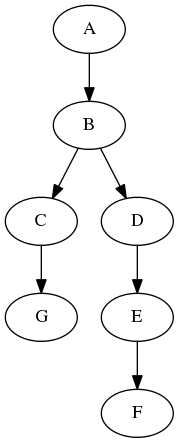
\includegraphics[scale=0.4]{imgs/tree1.png}
  \caption{Note que os nós (predicados) A, E, G e F são irrelevantes e podemos tira-los. Além disso
  o nó B deve ser o primeiro predicado a ser perguntado, já que este impacta mais na inferência.}
\end{figure}

\section{Prolog}

\paragraph{
  Prolog é uma linguagem bem diferente das quais estou acostumado. Por ser uma linguagem onde lidamos
  com fatos e regras ao invés de ser uma linguagem procedimental e imperativa como C, demorou um
  tempo para acostumar-se. No entanto, é uma experiência diferente e muito interessante.
}

\section{Desempenho}

\paragraph{
  O programa conseguiu acertar todas as vezes o personagem. No entanto, para certos personagens,
  se o usuário erra uma das características dele, o programa imprime como certo. Por exemplo, se
  acertarmos que \texttt{flynn\_white} tem as características \texttt{is\_male}, \texttt{is\_teenager},
  \texttt{has\_daddy\_issues} mas errarmos e dissermos que ele \texttt{is\_bold}, o programa dirá
  que o personagem escolhido foi \texttt{flynn\_white} ao invés de \texttt{unknown}.
}

\paragraph{
  Com relação a perguntas em média, o programa conseguia decidir qual o personagem escolhido com
  cinco perguntas em média. Além disso, é interessante notar que os personagens que estavam antes
  na lista de declaração de regras, foram os que obtiveram menor número de perguntas para serem
  adivinhados. Além disso, aqueles que possuíam características compartilhadas com um pequeno número
  de personagens tinham maior média de perguntas.
}

\section{Melhorias}

\paragraph{
  Como vimos na seção Predicados Ideais e Desempenho, mudar a ordem dos predicados é um jeito de
  melhorarmos a performance do programa. Além disso, formular predicados que sejam compartilhados
  com um maior número de personagens também, já que podemos excluir aqueles que admitem tal característica
  daqueles que não admitem em maior quantidade, e portanto limitaremos o conjunto de possíveis respostas
  mais rapidamente. Outro jeito, mais óbvio, de melhorar o programa seria descartar todos os predicados
  desnecessários, ou seja, que não alterem o resultado da query.
}

\section{Notas}

\paragraph{
  Nas linhas 2 e 18 do código, tentei melhorar o jeito de se adicionar fatos a base de conhecimento.
  Minha intenção era colocar todos os personagens numa lista e para cada membro, adicionar o fato:
}

\begin{equation}
  guess(X) :- X,!.
\end{equation}

\paragraph{
  Infelizmente meu conhecimento de Prolog é muito ruim e isso não funciona. :(
}

\end{document}
